% !TEX root = ../main.tex

\chapter{三角贝赛尔曲面片表示的光滑自由变形概述}
光滑自由变形算法基于精确自由变形\cite{Feng98},并在此基础上做了如下改进:

\begin{itemize}
    \item 同时考虑待变形模型的几何信息和法向信息,利用法向信息调整变形结果,使最终的变形结果在光滑边两侧具有视觉上$G^1$连续的几何和$G^0$连续的法向量场;在尖锐边两侧具有$G^0$连续的几何和$G^{-1}$连续的法向量场。
        \item 利用GPU实现变形过程中的算法,使用户在变形过程中与软件的交互能够实时进行。
\end{itemize}

光滑自由变形同样采用了自由变形算法框架,下文将沿着该框架的流程,对光滑自由变形算法进行简单介绍。

\section{定义变形空间}
光滑自由变形选用B样条体作为变形空间,记作$\mathbf R(u,v,w)$:
\begin{equation}
	\footnotesize
	{\mathbf R}(u,v,w) 
	= \sum_{i=0}^{m_u-1}\sum_{j=0}^{m_v-1}\sum_{k=0}^{m_w-1} {\mathbf R}_{ijk}N_{i,n_u}(u)N_{j,n_v}(v)N_{k,n_w}(w)
	\label{equ:Ruvw}
\end{equation}
其中,$n_u$、$n_v$、$n_w$与$m_u$、$m_v$、$m_w$分别表示B样条体三个维度上的次数与控制顶点个数。$\{\mathbf R_{ijk}\}_{i=0,\hspace{6 pt} j=0,\hspace{8 pt} k=0}^{m_u-1,m_v-1,m_w-1}$表示$m_u\times m_v\times m_w$个控制顶点。$\{N_{i,n_u}(u)\}_{i=0}^{m_u-1}$, $\{N_{j,n_v}(v)\}_{j=0}^{m_v-1}$ 和 $\{N_{k,n_w}(w)\}_{k=0}^{m_w-1}$是B样条基函数。

此B样条体三个维度上的节点向量分别是$\{u_i\}^{n_u+m_u}_{i=0}$, $\{v_i\}^{n_v+m_v}_{j=0}$ 和 $\{w_k\}^{n_k+m_k}_{k=0}$。由此定义的三维区域$[u_i, u_{i+1}] \times [v_j, v_{j+1}] \times [w_k, w_{k+1}]$我们称之为节点盒,其中$n_u\leq i < m_u$,$n_v\leq j < m_v$,$n_w\leq k < m_w$。


\subsection{沿节点盒切割多边形面片} \label{sec:clip_against_knot_box}
根据精确自由变形\cite{Feng98, Feng00},完全在某个节点盒内的三角面片,其变形后的结果是一个三角贝赛尔曲面片,记作${\mathbf P}(u,v,w)$:\label{section:split}

\begin{equation}
	\footnotesize
	{\mathbf P}(u,v,w)
	= \sum_{\substack{i+j+k=n \\ 0\leq i,j,k\leq n}} {\mathbf P}_{ijk}B^n_{ijk}(u,v,w), \hspace{8 pt} u,v,w\ge0,
		\hspace{8 pt}u+v+w=1
	\label{equ:Puvw}
\end{equation}

其中$\{B_{ijk}^n(u,v,w)=\frac{n!}{i!j!k!}u^iv^jw^k \mid i+j+k=n\}$是定义在一个三角形上的伯恩斯坦基函数,$n=n_u+n_v+n_w$为曲面片的次数,$\{\mathbf P_{ijk} \mid i+j+k=n\}$为些三角贝赛尔曲面片的$m=(n+1)(n+2)/2$个控制顶点。

所以由平面多边形构成的模型在嵌入B样条体之前,需要沿上述节点盒切割,且得到的非三角形的子多边形还需再进行三角化。以保证变形后的结果可以用三角贝赛尔曲面片表示。

如前方所述,在精确自由变形中,最终的作为变形结果的三角贝赛尔曲面片的次数会随着B样条体的增加而增加。所以变形结果往往是高次的曲面。

崔在工作中\cite{Cui15}发现,三次的曲面片已经能够提供足够的灵活度来表示各种变形结果。精确自由变形中所用的高次曲面片,虽然得到了精确的结果,但同时也带来了很高的计算代价。因此,光滑自由变形采用次数为三次的三角贝赛尔曲面片来拟合高次的精确结果。以很小的拟合误差换取了较大的性能提升。

综上,在光滑自由变形中,沿节点盒切割并不能保证结果是精确的。但同时崔也尝试了省略这一步骤,直接进行变形拟合。结果较小的三角形或位于唯一结点盒内的三角形,其拟合误差不会显著增加,但是较大的跨多个节点盒的三角形会产生较大的拟合误差。所以在光滑自由变形中仍然保留沿节点盒切割这一步骤,但是该步骤的目的不再是保证结果精确,而是减小三角形面积以降低拟合误差。这也是本文用新的三角剖分算法替代沿节点盒切割的算法的理论基础。

切割多边形面片实际上是平面求交问题。此类问题在现实中的解空间是连续的,而当问题被描述成具体的算法时,其解空间却是离散的。所以节点盒切割算法会因数值精度问题出现很多特殊情况,算法很难做到高效、鲁棒。另一方面切割本身也会产生很多狭长的三角形甚至蜕化三角形,这些三角形不尽会浪费计算资源,还会给后续计算带来不便。

因此本文将会提出新的分割算法以解决以上两方面的问题。

\section{模型嵌入变形空间}
“嵌入”过程,其实是计算“待变形的对象”在变形空间中的参数坐标的过程。从用户角度来看,“侍变形对象”就是待变形的模型;但是从算法实现的角度来看,真正参与变形的实际上是模型上的采样点。因此,“嵌入”就是通过嵌入函数$U=E(X)$将采样点从笛卡尔坐标系映射到变形空间的过程。其中$X$为采样点在笛卡尔坐标系中的坐标,$U$为采样点在变形空间的参数坐标。

所以嵌入变形空间这一过程有两个要点:确定变形函数、选取采样点。

\subsection{确定变形函数}
嵌入函数$E(X)$由变形空间决定。光滑自由变形通过\cite{Feng02}中的方法构造B样条体,使得其具有如下性质:嵌入变形空间的点的参数坐标与该点在世界坐标系中的坐标相等,即$E(X)=X$。

\subsection{采样点的选取}
不同的种类的FFD算法,需要选取不同的采样点。

传统自由变形常常以待变形模型的顶点为采样点,这将导致如图\autoref{fig:sample_problem}所示的走样问题。均匀加密采样只能在一定程度上解决走样问题,且随着采样点密度的增加,无论是时间还是空间上的开销均会显著增加。自适应的加密采样是在加密采样思路下解决走样问题的更进一步的尝试。相对均匀加密采样而言,其虽然能减少一定计算量,但是实现复杂,无法很好的应对一些特殊情况。以上两种方法匀无法从根本上解决走样问题。

精确自由变形\cite{Feng00}则通过另一种思路从根本上解决了走样问题。如\ref{section:split}所述,三角面片变形后是一个三角贝赛尔曲面片,所以,只要用FFD求得三角面片上的$m$(控制顶点数)个均匀采样点在变形之后的位置,就可以通过多项式插值高效计算出三角贝赛尔曲面片的控制顶点。这一方法相对于加密采样的优势在于其结果是一个解析表达的贝赛尔曲面片,可以根据需求细化绘制出不同精度的变形结果,而无需改变采样点个数。

光滑自由变形\cite{Cui15}进一步优化了精确自由变形的计算量。首先,崔指出在精确自由变形中作为变形结果的三角贝赛尔曲面片,其次数往往高于三次,高次的结果不仅会直接产生高昂的计算代价,还会间接的增加算法其它部分的复杂度。然后,崔通过实验发现,三次的三角贝赛尔曲面片能提供足够的灵活性以拟合精确的自由变形结果。所以,崔选用了三次贝赛尔曲面片来表示变形结果。该曲面片由带约束的拟合方法求出,该方法需要$3\times3$个约束点,$m$个拟合点。所以,光滑自由变形共需要$9+m$个采样点。\autoref{fig:saffd_sample_point}中展示了当次数为4时,采样点的选取方式,黄色点为约束点,蓝色点为拟合点。三角形三个顶点既是约束点又是拟合点,图中略微错开以表示区别,实际上是同一个点。

\begin{figure}[htbp]
	\centering
	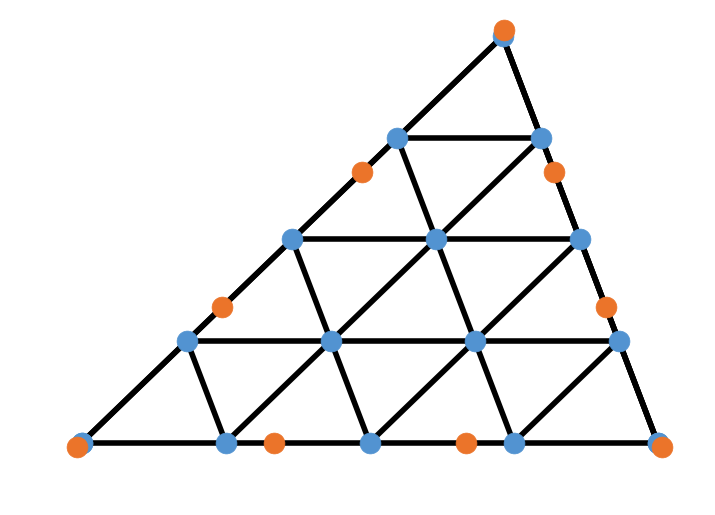
\includegraphics[width = 0.5\linewidth]{saffd_sample_point.png}
    \caption{三角面片上的拟合点的约束点示意图}\label{fig:saffd_sample_point}
\end{figure}


\section{变形}
\subsection{几何变形}
变形过程实际上就是改变变形空间,并将变形“传递”到待变形模型的过程。通过前文所述的步骤,我们已经将采样点嵌入到B样条体中。算法就是通过这些采样点将变形“传递”到待变形模型中的。当用户编辑B样条体控制顶点的位置后,算法先将采样点的参数坐标和控制顶点位置代入\autoref{equ:Ruvw},就可以求得采样点变形后的位置。再以这些采样点新的位置为输入,通过带约束的拟合方法,求出作为变形结果的三角贝赛尔曲面的控制顶点。\autoref{subfig:sffd_0}是原模型,\autoref{subfig:sffd_1}是将上述变形得到的三角贝赛尔曲面片细分成三角形后进行绘制的结果,绘制时所用的法向由三角形边向量叉乘得到。

\begin{figure}[htbp]
	\centering
	\begin{subfigure}[b]{.4\textwidth}
		\centering
		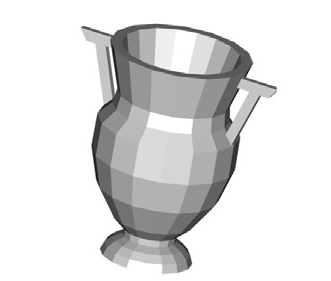
\includegraphics[width = \textwidth]{sffd_0.png}
		\caption{原模型}\label{subfig:sffd_0}
	\end{subfigure}
	\quad
	\begin{subfigure}[b]{.4\textwidth}
		\centering
		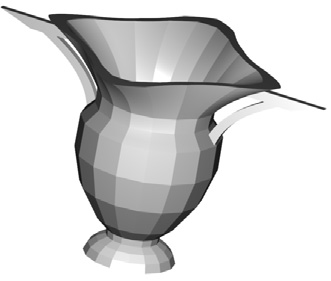
\includegraphics[width = \textwidth]{sffd_1.png}
		\caption{几何变形结果}\label{subfig:sffd_1}
	\end{subfigure}
    \caption{光滑自由变形示意图}\label{fig:sffd}
\end{figure}

\subsection{法向变形}
因为上述过程并未考虑模型的法向信息,可以很明显的看出\autoref{subfig:sffd_1}中的结果并不光滑。为了改进这一点,光滑自由变形将法向也纳入了变形构架中。首先我们通过重心坐标插值求得采样点的法向,然后通过Gain\cite{gain1999}的方法计算出采样点的法向量变形以后的位置。接着,用与几何变形中相同的方法,以采样点的变形后的法向量为输入,我们就可以用三次贝赛尔曲面片拟合出变形后的三角面片法向量场。在细分阶段我们同时细分法向量场,并以此作为细分三角形的法向,这样的我们就有了在光滑边两侧视觉上$G^1$连续的几何和$G^0$连续的法向量场;在尖锐边两侧$G^0$连续的几何和$G^{-1}$连续的法向量场。\autoref{subfig:sffd_smooth_0}展示了加入法向信息后的变形结果。

\begin{figure}[htbp]
	\centering
	\begin{subfigure}[b]{.4\textwidth}
		\centering
		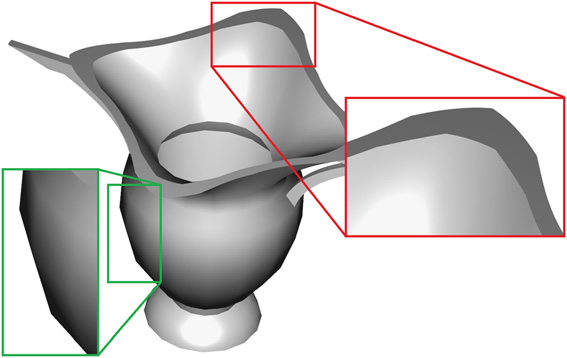
\includegraphics[width = \textwidth]{sffd_smooth_0.png}
		\caption{变形结果}\label{subfig:sffd_smooth_0}
	\end{subfigure}
	\quad
	\begin{subfigure}[b]{.4\textwidth}
		\centering
		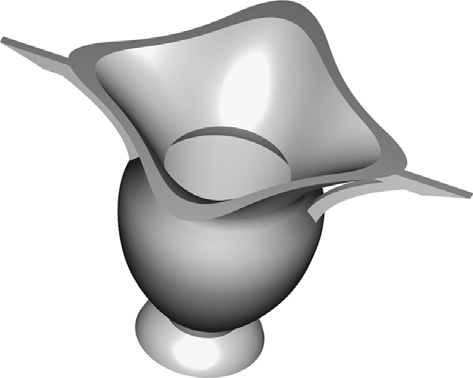
\includegraphics[width = \textwidth]{sffd_smooth_1.png}
		\caption{变形结果}\label{subfig:sffd_smooth_1}
	\end{subfigure}
    \caption{光滑自由变形示意图}\label{fig:sffd}
\end{figure}

\section{几何微调}
\autoref{subfig:sffd_smooth_0}中的结果,尽管着色结果很光滑,但是几何方面仍然存在走样。\autoref{subfig:sffd_smooth_0}中的框出来的部分,红色部分和绿色部分分别体现了尖锐边界和侧影轮廓线的走样。为了解决这些问题,得到视觉上更加细腻的变形结果,算法还将根据法向信息对表示几何的三角贝赛尔曲面片的控制顶点进行了微调。最终输出光滑并保持尖锐特征的结果,\autoref{subfig:sffd_smooth_1}所示。

以上就是光滑自由变形的大致步骤,其算法流程如\autoref{fig:algorithm_sffd}所示,在下文将介绍本文算法在此基础上进行的改进。


\tikzstyle{GPU} = [rectangle, draw, fill=blue!15, 
    text width=15em, text centered, rounded corners, minimum height=3em]

\tikzstyle{CPU} = [rectangle, draw, fill=red!15, 
    text width=15em, text centered, rounded corners, minimum height=3em]
\tikzstyle{line} = [draw, thick, ->, >= stealth]

\begin{figure}
	\centering

    \begin{tikzpicture}[node distance = 2cm, auto]
        % Place nodes
        \node [CPU] (read) {1、输入多边形网格模型,并三角化};
        \node [CPU, below of=read] (initspace) {2、初始化B样条空间};
        \node [GPU, below of=initspace] (pntriangle) {3、求子三角面片的PN-Triangle,用以调整变形结果};
        \node [CPU, below of=pntriangle] (split) {4、根据结点盒切割多边形};
        \node [GPU, below of=split] (sample) {5、根据控制顶点,计算采样点的位置与法向};
        \node [GPU, below of=sample] (deformation) {6、用带约束的拟合的方法,计算出三角贝赛尔曲面片和法向量场的控制顶点};
        \node [GPU, below of=deformation] (adjust) {7、用法向信息和PN-Triangle信息调整上一步得到的控制顶点};
        \node [GPU, below of=adjust] (tess) {8、细分变形结果并绘制};
        \node [CPU, right=2em of deformation] (edit) {9、用户编辑控制顶点};

        % Draw edges
        \path [line] (read) -- (initspace);
        \path [line] (initspace) -- (pntriangle);
        \path [line] (pntriangle) -- (split);
        \path [line] (split) -- (sample);
        \path [line] (sample) -- (deformation);
        \path [line] (deformation) -- (adjust);
        \path [line] (adjust) -- (tess);
        \path [line] (tess) -| (edit);
        \path [line] (edit) |- (sample);
    \end{tikzpicture}

    \caption{本文算法流程图\\红色框表示在CPU中运行,蓝框表示在GPU中运行}\label{fig:algorithm_sffd}
\end{figure}
